\chapter{Diseño}
\label{cap:capitulo4}

Tras haber puesto en contexto todo lo anterior, en este capítulo se expondrá, de forma detallada, el proceso seguido para conseguir que un dron detecte y navegue hacia una señal \ac{RF}.\\

Además, se mostrará el desarrollo de una aplicación responsiva, que simula el comportamiento de una señal (en un espacio libre de obstáculos), basada en la aproximación de Friis.\\

Por último, se buscará determinar cuál de los métodos empleados es mejor y por qué, a través de diversas métricas comparativas que se expondrán en detalle posteriormente.\\

\section{Preparación del entorno}
\label{sec:preparacion_del_entorno}

Lo primero que se debía conseguir, era un entorno de simulación compatible con \ac{ROS}, así como un sistema de control de versiones, que nos permitiera mantener la trazabilidad y los backups a mano. Por ello, se estableció un repositorio común en \textbf{GitHub} y se empleó el paquete de herramientas dispuesto por \textbf{JdeRobot}.

\subsection{JdeRobot - drones}
\label{subsec:jderobot_drones}

Gracias a esta plataforma, se pudieron obtener los modelos y los módulos necesarios para simular en Gazebo 11 el desempeño de un cuadracóptero, provisto de un sistema autopilot PX4.\\
\newpage
El modelo usado es el \textbf{3DR Iris simulado}, con un plugin de una cámara frontal. Este dispositivo utiliza MAVROS para realizar la comunicación, lo que nos permite enviar y recibir mesajes ROS compatibles con el protocolo de comunicaciones típico de estas aeronaves, MAVLink.\\

\begin{figure} [H]
	\begin{center}
	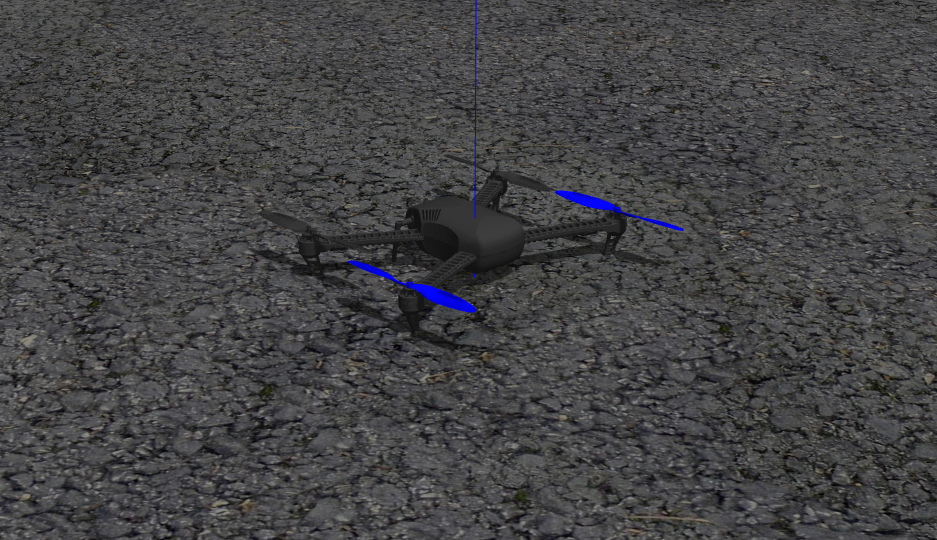
\includegraphics[height=4cm]{imagenes/cap4/1_px4_drone_gz.png}
	\end{center}
	\caption[3DR Iris simulado]{3DR Iris simulado}
	\label{fig:3dr_iris}
\end{figure}

\subsection{Teleoperador}
\label{subsec:teleoperador}

Ya propiamente hablando de resolver el problema planteado, la primera aproximación propuesta fue hacer una interfaz gráfica simple, que permitiera enviar órdenes a la aeronave.\\

Para ello, inicialmente se debía conseguir enviar mensajes de forma programática. Por tanto, se diseñó un \textbf{script controlador} encargado de la comunicación directa con el \textbf{controlador de la aeronave}, para enviar y recibir diversos datos vía MAVROS. De igual modo, se debían satisfacer una serie de requisitos que aseguraran el correcto funcionamiento del sistema:

\begin{enumerate}
	\item La comunicación debe darse a \textbf{más de 2Hz}, para evitar cambios indeseados en el funcionamiento interno del controlador PX4 (de la aeronave).

	\item Antes de realizar cualquier comunicación, \textbf{debe asegurarse que el estado es \emph{``connected''}}, lo que significa que el dron esta armado y en modo \emph{OFFBOARD} (nuestra aeronave posee 7 modos distintos, \emph{HOLD}, que mantiene la posición, \emph{RETURN}, que vuelve al punto de despegue, \emph{MISSION}, que permite cargar rutas programadas con anterioridad, \emph{TAKEOFF}, habilita el despegue, \emph{LAND}, habilita el aterrizaje, \emph{FOLLOW ME}, que permite seguir objetivos, y \emph{OFFBOARD}, que permite comandar al dron sin necesidad de GPS, lo que es útil de cara al desarrollo de aplicaciones robóticas) \cite{flight-modes}.
	
    \item Una vez esta conectado, se deben \textbf{enviar datos} (velocidades en nuestro caso) al controlador PX4, con el fin de \textbf{evitar el cierre de la conexión}. Estos datos carecen de utilidad más que la de asegurar dicha conectividad.
    
    \item Por último, y antes de enviar cualquier posición, velocidad o comando (distintos modos de actuación), se debe comprobar siempre que el \textbf{modo activo} es \emph{OFFBOARD} y que el dron esta \textbf{armado} (listo para volar). En caso contrario, se debe solicitar al controlador, mediante servicios, dichas especificaciones.
\end{enumerate}

Por tanto, con todo esto funcionando de forma correcta, la manera de generar comportamientos en el dron en sí, es mediante \emph{topics}. Concretamente, los que genera MAVROS automáticamente cuando se lanza todo el sistema. Tal y como se comentó en apartados previos, estos \emph{topics} sólo admiten mensajes \ac{ROS}, lo que encapsula el mensaje real transmitido al controlador PX4, que solo es compatible con MAVLINK.\\

En nuestro caso, enviaremos posiciones (PoseStamped), velocidades (Twist) y comandos (sevicios formados por mensajes personalizados, creados por MAVROS, con formato \ac{ROS}). Esto, nos permitirá conectar el resto de aplicaciones con el script controlador, mediante \emph{topics} comunes, de forma que se encargue de enviar la acción final al dron, mientras el resto de scripts se encarguen de resolver otras tareas.\\

De este modo, inicia el desarrollo propiamente dicho del \textbf{teleoperador}. El teleoperador, se diseñó con el fin de generar comportamientos que se usarían en las fases finales del \ac{TFG}. Sin embargo, en la primera versión, tan solo se buscó construir una interfaz gráfica sencilla, capaz de enviar ordenes usando \ac{ROS} que, en última instancia, llegasen al dron y produjesen diversos comportamientos, tales como \textbf{moverse y girar}, a través de sliders.\\

\begin{figure} [H]
	\begin{center}
	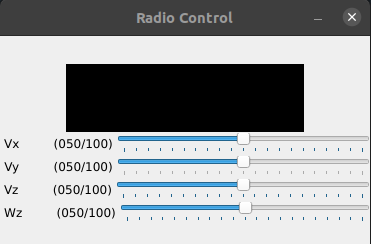
\includegraphics[height=4.5cm]{imagenes/cap4/2_axes_rc.png}
	\end{center}
	\caption[Primera versión del teleoperador]{Primera versión del teleoperador}
	\label{fig:teleoperador_v1}
\end{figure}

En el siguente paso, se buscó programar \textbf{comportamientos predefinidos}, es decir, acciones predeterminadas tales como desplazarse distancias concretas en ciertas direcciones, o girar un número específico de grados en un sentido u otro. Para ello, se diseñó una ampliación sobre la interfaz anterior, en la que se añadió un \textbf{botón por cada acción} concreta desarrollada, además de una \textbf{imagen de la cámara frontal} en directo. Es importante destacar la acción de moverse de distancias específicas, ya que se empleará en los algoritmos posteriores.\\

Finalmente, y continuando con lo anterior, se intentó afinar el comportamiento de las acciones predefinidas, para hacer que el dron se desplazase de celda en celda, concretamente de \textbf{centro en centro}. La idea es que, el dron solo tomará medidas de la señal en posiciones concretas y no en movimiento. Además, se agregaron \textbf{marcadores en \emph{rviz}}, para determinar las celdas visitadas (con colores aleatorios), junto con otro marcador que muestra la trayectoria que sigue la aeronave.\\

\begin{figure} [H]
	\begin{center}
	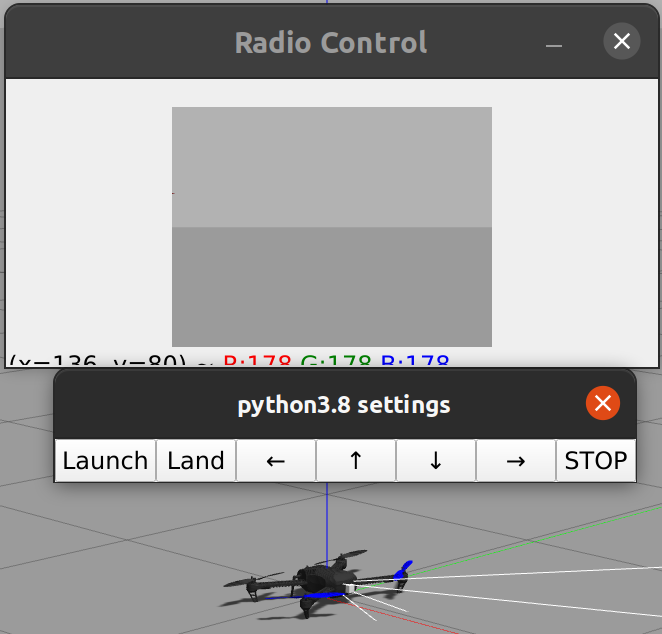
\includegraphics[height=8cm]{imagenes/cap4/3_c2c_gui.png}
	\end{center}
	\caption[Versión final del teleoperador]{Versión final del teleoperador}
	\label{fig:teleoperador_end}
\end{figure}

\newpage
A continuación, se muestra el \emph{``main''} de la aplicación mencionada:\\

\begin{code}[H]
\begin{lstlisting}[language=Python]
if __name__ == '__main__':
    try:
        rospy.init_node(NODENAME, anonymous=True)

        # Msgs
        ## Subscribers
        image_sub = rospy.Subscriber(IMAGE_TOPIC, Image, callback = image_cb)
        current_pos_sub = rospy.Subscriber(LOCAL_POSE_TOPIC, PoseStamped, callback = current_pos_cb)

        ## Publishers
        pos_pub = rospy.Publisher(RADIO_CONTROL_POS_TOPIC, PoseStamped, queue_size=10)
        cmd_pub = rospy.Publisher(RADIO_CONTROL_CMD_TOPIC, Px4Cmd, queue_size=10)

        # -- OPENCV -- #
        cv2.namedWindow(WINDOWNAME)

        # Buttons
        cv2.createButton('Launch', launch_button, None, cv2.QT_PUSH_BUTTON, 1)
        cv2.createButton('Land', land_button, None, cv2.QT_PUSH_BUTTON, 1)
        cv2.createButton('←', left_button, None, cv2.QT_PUSH_BUTTON, 1)
        cv2.createButton('↑', front_button, None, cv2.QT_PUSH_BUTTON, 1)
        cv2.createButton('↓', back_button, None, cv2.QT_PUSH_BUTTON, 1)
        cv2.createButton('→', right_button, None, cv2.QT_PUSH_BUTTON, 1)
        cv2.createButton('STOP', stop_button, None, cv2.QT_PUSH_BUTTON, 1)

        cv2.waitKey(0)
        cv2.destroyAllWindows()
    except rospy.ROSInterruptException:
        pass
\end{lstlisting}
\caption[Main de center to center app]{Main de center to center app}
\label{cod:c2c_app}
\end{code}

Donde, tras inicializar el nodo \ac{ROS}, se definen por un lado los \textbf{suscriptores}, encargados de recibir los datos de la cámara y la posición del dron (usando MAVROS), los \textbf{publicadores}, cuya función es enviar posiciones y/o comandos al script controlador, y por último la \textbf{interfaz gráfica} diseñada con \textbf{OpenCV}, donde se define la ventana y los botones con las diversas acciones predefinidas \footnote{Código completo en \url{https://github.com/RoboticsLabURJC/2022-tfg-cristian-sanchez/blob/main/src/teleop/scripts/c2c_control.py}}.\\

\section{Señales}
\label{sec:signals}

Continuando con el proyecto, entramos en el segundo gran bloque, las \textbf{señales \ac{RF}}. Este apartado fue especialmente relevante, ya que nos permitió desarrollar una aplicación reactiva, con la meta de generar entornos sobre los que probar soluciones robóticas.\\

Pero, antes de entrar en detalle en estos aspectos, conviene familiarizarse con algunos \textbf{conceptos básicos} sobre el \textbf{procesamiento de señales}:

\begin{enumerate}
	\item \emph{Señal}: se trata de una función que describe un fenómeno físico, y que se emplea para la transmisión de información.
	
    \item \emph{Dominio temporal}: establece el eje de abcisas con el tiempo. 
    
    \item \emph{Dominio de la señal}: determina si la señal se expresa en tiempo o en frecuencia (a través de transformadas).
    
    \item \ac{ADC}: elemento electrónico que permite la conversión de señales analógicas a señales digitales.
    
    \item \ac{RSSI}: permite establecer el nivel de potencia de una señal, con respecto a 1 mW de potencia. Se expresa en dBm.
    
    \item \ac{SNR}: métrica que permite medir la potencia de la señal con respecto al ruido ambiente.

    \item \emph{Frecuencia}: parámetro de la función que define a la señal, el cual determina el número de veces que se repite en un segundo. Se mide en hercios (Hz).
    
    \item \emph{TX}: Se refiere a la transmisión de la señal.
    
    \item \emph{RX}: Hace referencia a la recepción de la señal.
\end{enumerate} \cite{basics-signals}\\

Definidos estos términos, nuestro objetivo se basó en obtener un modelo capaz de calcular la \textbf{propagación de la señal}, es decir, un sistema capaz de calcular como se comporta la potencia de una señal, según las características de su entorno.\\

\subsection{Aproximación de Friis}
\label{subsec:friis}

Por ello, se optó por emplear la aproximación de Friis, que nos proporciona una sencilla fórmula sobre la cual modelizar nuestro problema:

\begin{align}
    P_r = P_t \cdot \left( \frac{G_t G_r \lambda^2 }{(4 \pi)^2 d^n L} \right)
\end{align}

Donde cada término significa lo siguiente:

\begin{enumerate}
    \item \emph{$P_t$ y $P_r$}: aluden a la potencia del transmisor y la potencia del receptor respectivamente.

    \item \emph{Ganancias} ($G_t$, $G_r$): representan un valor incremental aplicado a la potencia de emisión y de recepción, respectivamente.
    
    \item \emph{Valor lambda} ($\lambda$): hace referencia a la longitud de onda. Está directamente relacionado con la frecuencia.
    
    \item \emph{Distancia} (d): desde el origen de la señal a un punto en el espacio.
    
    \item \emph{L}: representa todas aquellas pérdidas no asociadas a la propagación de la señal.
    
    \item \ac{PLE} (n): permite ajustar el modelo a diversos entornos. Es un valor constante extraido de forma empírica. A continuación se muestra una tabla con varios ejemplos.
\end{enumerate} \cite{friis-1}\\

\begin{figure} [H]
	\begin{center}
	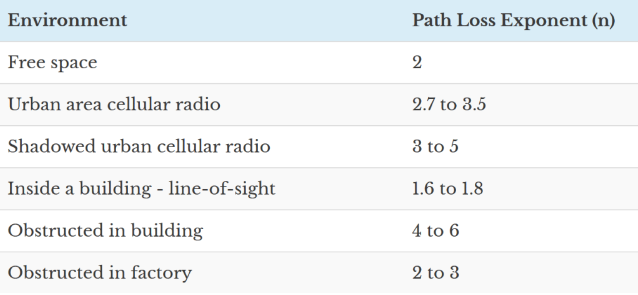
\includegraphics[height=5cm]{imagenes/cap4/4_PLE_table.png}
	\end{center}
	\caption[Tabla ejemplos exponente n]{Tabla ejemplos exponente n}
	\label{fig:ple_table}
\end{figure}

Además, empleando este método, podemos modelizar las \textbf{pérdidas de una señal} estimadas durante su propagación, a través de la siguiente ecuación:\\

\begin{align}
    P_L(dB) = -10 \log_{10} \frac{\lambda^2}{(4 \pi d)^2} 
\end{align}

Sin embargo, para nuestro caso no es relevante (aunque está incluido dentro del módulo).\\

\subsection{Módulo python de Friis}
\label{subsec:friis-module}

Una vez realizadas las pruebas iniciales, se buscó compactar todo, de forma que fuera accesible para cada aplicación que lo necesitase.\\

Por ello, surgió la idea de crear un \textbf{módulo python} que se encargará de modelizar las ecuaciones previamente mencionadas. Para ello, se diseño una clase cuyo constructor se encargara de recibir, por parámetros, las variables implicadas en las ecuaciones de Friis, además de las dimensiones del mapa y su resolución (la cual afecta al tamaño de celda).\\

Básicamente, el \textbf{proceso} seguido para usar este módulo es el siguiente, primero se crea un objeto de la clase Friis donde se especifican las características de la señal y las variables relacionadas con el mapa, lo que genera internamente un array 2D vacío, que será rellenado en función del modelo seleccionado. Posteriormente, se selecciona el modelo deseado (propagación o pérdidas, este último no está testeado), pasando las coordenadas del origen de la señal por parámetros. Esto, retornará el mapa relleno con los valores asociados a las ecuaciones del modelo de Friis seleccionado.\\

A continuación se mostrará un ejemplo sencillo de uso, donde se obtendrá un mapa de propagación de señal, en forma de Numpy array 2D:

\begin{code}[H]
    \begin{lstlisting}[language=Python]

    #! /usr/bin/env python    
    import friss as fr

    if __name__ == '__main__':
        friis_object = fr.Friss(power_tras=10.0, 
                                gain_tras=1.5, 
                                gain_recv=2.0,
                                freq=fr.FREQ_WIFI, 
                                losses_factor=1.0, 
                                losses_path=2.0,
                                world_sz=(10,10), 
                                resolution=1.0)

        signal_map = friis_object.model_power_signal(origin=(5,3))

\end{lstlisting}
\caption[Ejemplo básico de uso del módulo Friis]{Ejemplo básico de uso del módulo Friis}
\label{cod:friis_basics}
\end{code}

Yendo al detalle, se puede ver que se genera un mapa 10x10 con resolución 1 (es decir, cada celdilla es de 1x1 unidades), de una señal WIFI, donde el transmisor emite a 10 W, con una ganancia de 1.5, el receptor posee una ganancia de 2, un factor de pérdidas (L) de 1, es decir, sin pérdidas, y por último, el exponente n (\ac{PLE}) con un valor de 2, que representa el espacio vacío. Luego se genera el mapa de propagación de la señal, indicando que la fuente se encuentra en las coordenadas (5,3).\\

No obstante, este módulo posee \textbf{otras funcionalidades} útiles para trabajar con él, como son:

\begin{enumerate}
    \item \textbf{\emph{reset\_world}}: modifica el mapa que hubiera, estableciendo todos sus valores a cero.
    
    \item \textbf{\emph{get\_world\_sz}}: retorna las dimensiones del mapa.
    
    \item \textbf{\emph{set\_values}}: modifica las características de la señal simulada.
\end{enumerate}

Hay que tener en cuenta que, aunque se modifiquen los parámetros, se debe modelar de nuevo el mapa para que surtan efectos los cambios.\\
\newpage
Por último, se busco \textbf{extender la funcionalidad del módulo}, de manera que fuera posible incluir obstáculos en el mapa. La idea era crear un método capaz de posicionar \textbf{obstáculos} en el mapa de la señal, y simular su efecto en la señal.\\

Para ello, se buscó trazar proyecciones desde la señal hasta los bordes del obstáculo, de forma que se generase un polígono con los bordes del mapa. Posteriormente, se revisó que puntos se encontraban dentro del polígono (que no fueran propiamente parte del obstáculo), a través de un algoritmo basado en el número de intersecciones del punto con el perímetro del polígono, trazando una línea horizontal y hacia la derecha \cite{poly-info}. Por último, para cada punto dentro del polígono se le aplicó un factor de pérdida al valor almacenado de la señal, de manera que se simulase el efecto del obstáculo.\\

\begin{figure} [H]
	\begin{center}
	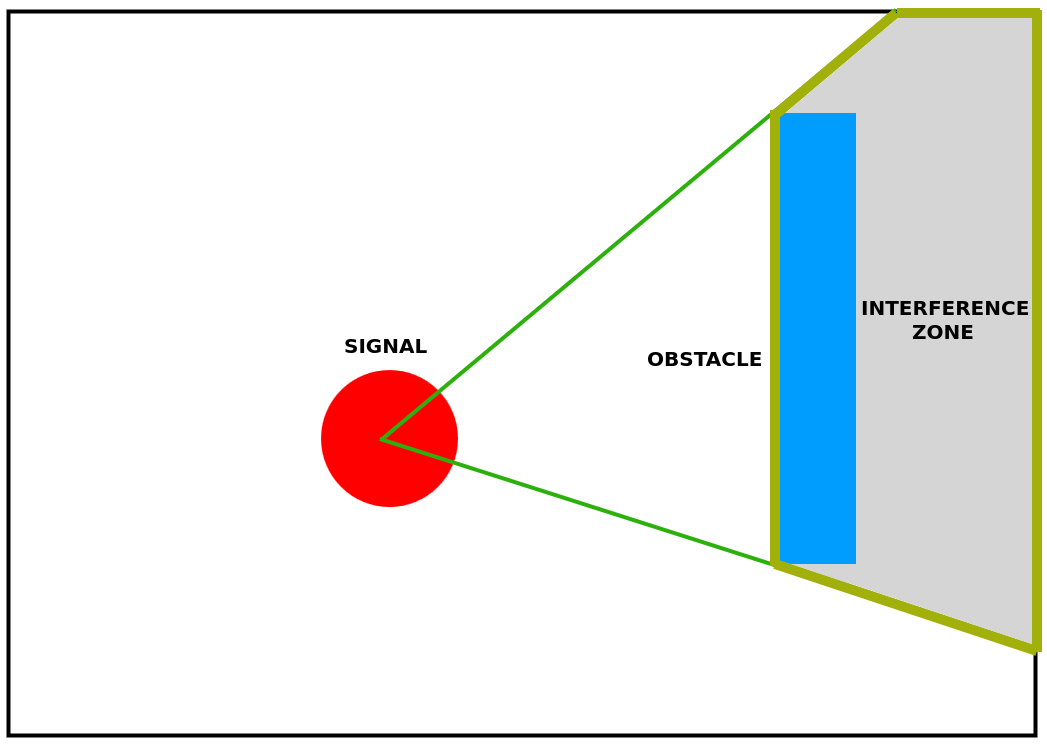
\includegraphics[height=7cm]{imagenes/cap4/5_interference.png}
	\end{center}
	\caption[Representación del algoritmo]{Representación del algoritmo}
	\label{fig:interference_algorithm}
\end{figure}

La idea fue abrir puertas a nuevos entornos más complejos y realistas, sobre los que poder probar diversas soluciones, en nuestro caso, para testear el efecto de un muro en el camino del dron a la señal.\\

(CÓDIGO EJEMPLO OBSTACULOS !!!!!!!!!!!!!)\\

\subsection{Aplicación de Friis}
\label{subsec:friis-app}

La última sección relacionada con las señales se centro en integrar el módulo previo, en una \textbf{interfaz gráfica intuitiva para el usuario}. La idea era estudiar, en tiempo real, como evolucionaba la señal cuando alguno de sus parametros, en la ecuación de Friis, era modificado.\\

Para llevarlo a cabo, se empleó la librería \textbf{matplotlib}, debido a la enorme cantidad de herramientas de las que dispone, así como de su sencillez a la hora de crear nuevas aplicaciones. Funciona de manera que se generan eventos que son gestionados en \emph{``callbacks''}, es decir, se generan bucles asociados a dichos eventos, que reaccionan a cambios en la interfaz generada.\\

En nuestro caso, la \textbf{estructura base} consta de una figura, sobre la que se agregan todos los elementos, entre los que encontramos los mapas de calor o \emph{``heatmap''} en forma de plots, las barras de acción o \emph{``sliders''}, botones, entre otros elementos que se explicarán más adelante.\\

Inicialmente, se optó por representar un mapa de calor con una barra de color asociada a los distintos valores de la señal. Además, se integraron sliders correspondientes a cada valor presente en la ecuación de Friis, tal y como se muestra a continuación:\\

\begin{figure} [H]
	\begin{center}
	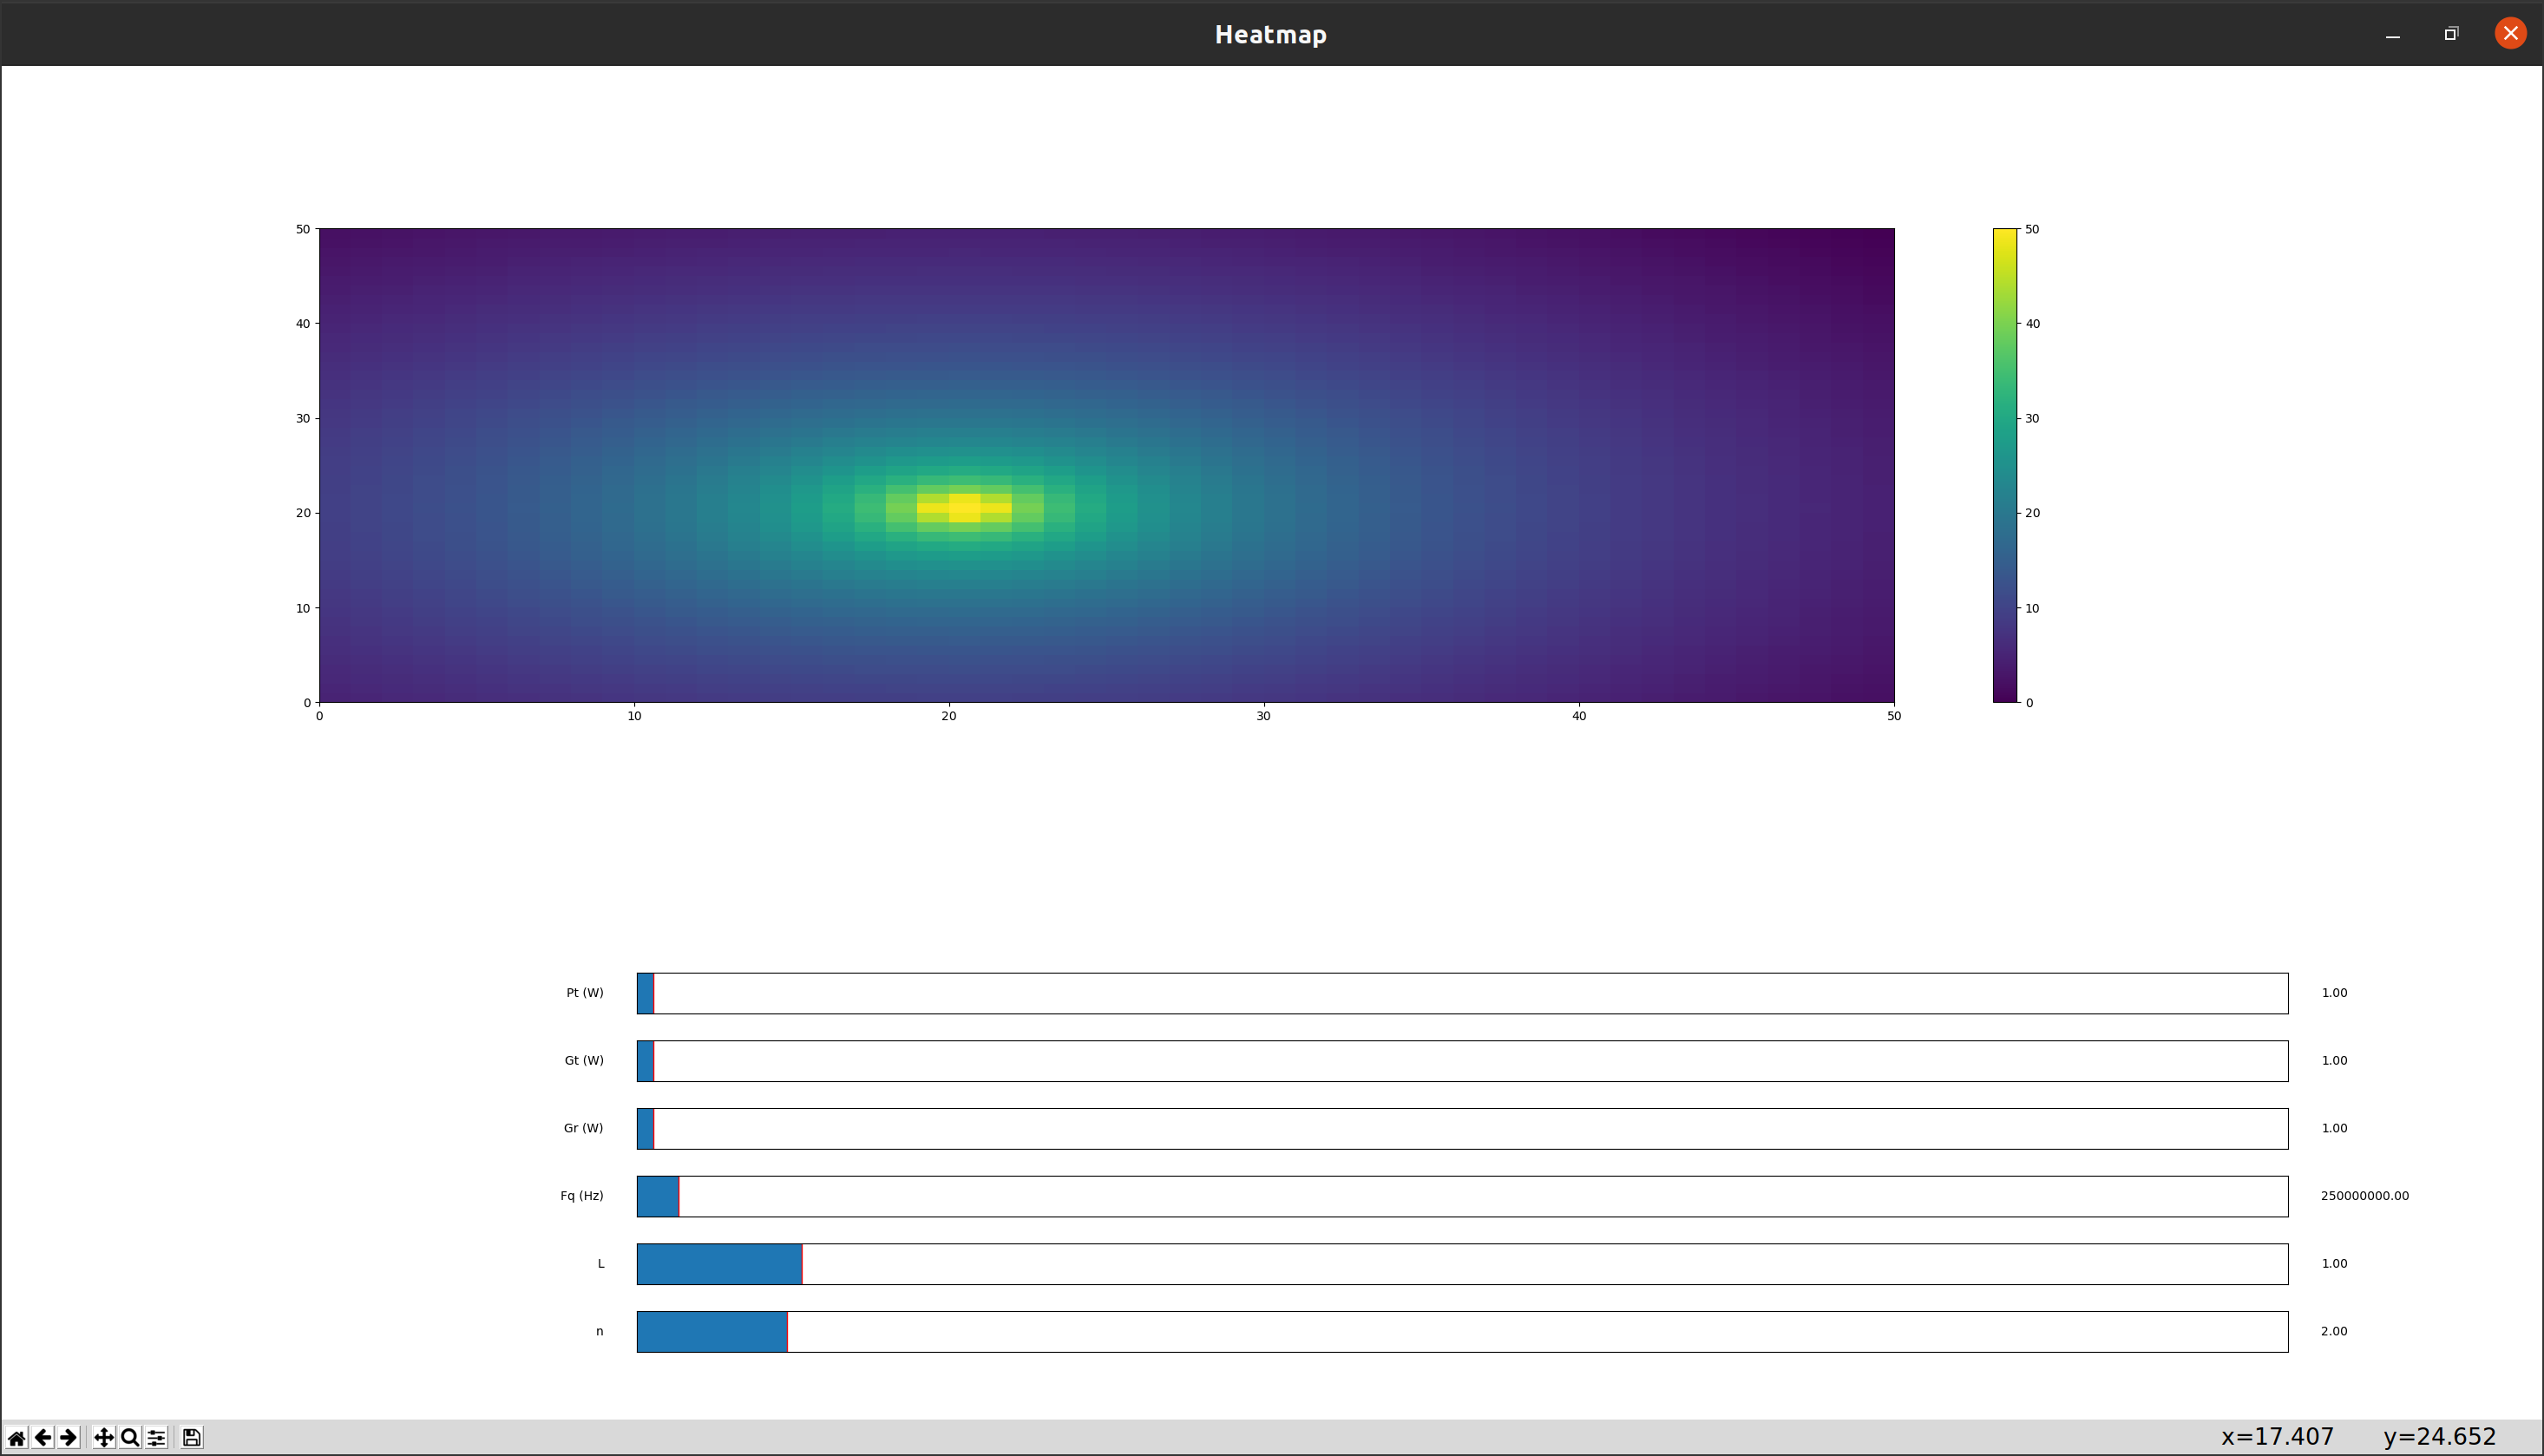
\includegraphics[height=8cm]{imagenes/cap4/6_Friss_firstGUI.png}
	\end{center}
	\caption[Primera versión de la interfaz]{Primera versión de la interfaz}
	\label{fig:friis_init_app}
\end{figure}
\newpage
El problema fue, que al actualizar los valores, también lo hacía la representación, por lo que no se apreciaba el efecto de los cambios en el plot.\\

Por ello, se agregaron dos mapas de calor, uno con el máximo y el mínimo fijados a mano (donde sí se aprecian los cambios), y el anterior mencionado. Para elegir cual usar, se agregó una casilla marcable. Además, se incluyeron dos variables relevantes a la hora de modelar, el \textbf{tamaño del mapa} y la \textbf{resolución}, manejadas a través de \emph{``sliders''}, los cuales a su vez se activan al pulsar un botón de \textbf{SET}, que recarga la interfaz. Además, se ajustó los saltos de valores para que fueran coherentes en el resto de barras de acción, tal y como se puede apreciar a continuación:\\

\begin{figure} [H]
    \begin{center}
    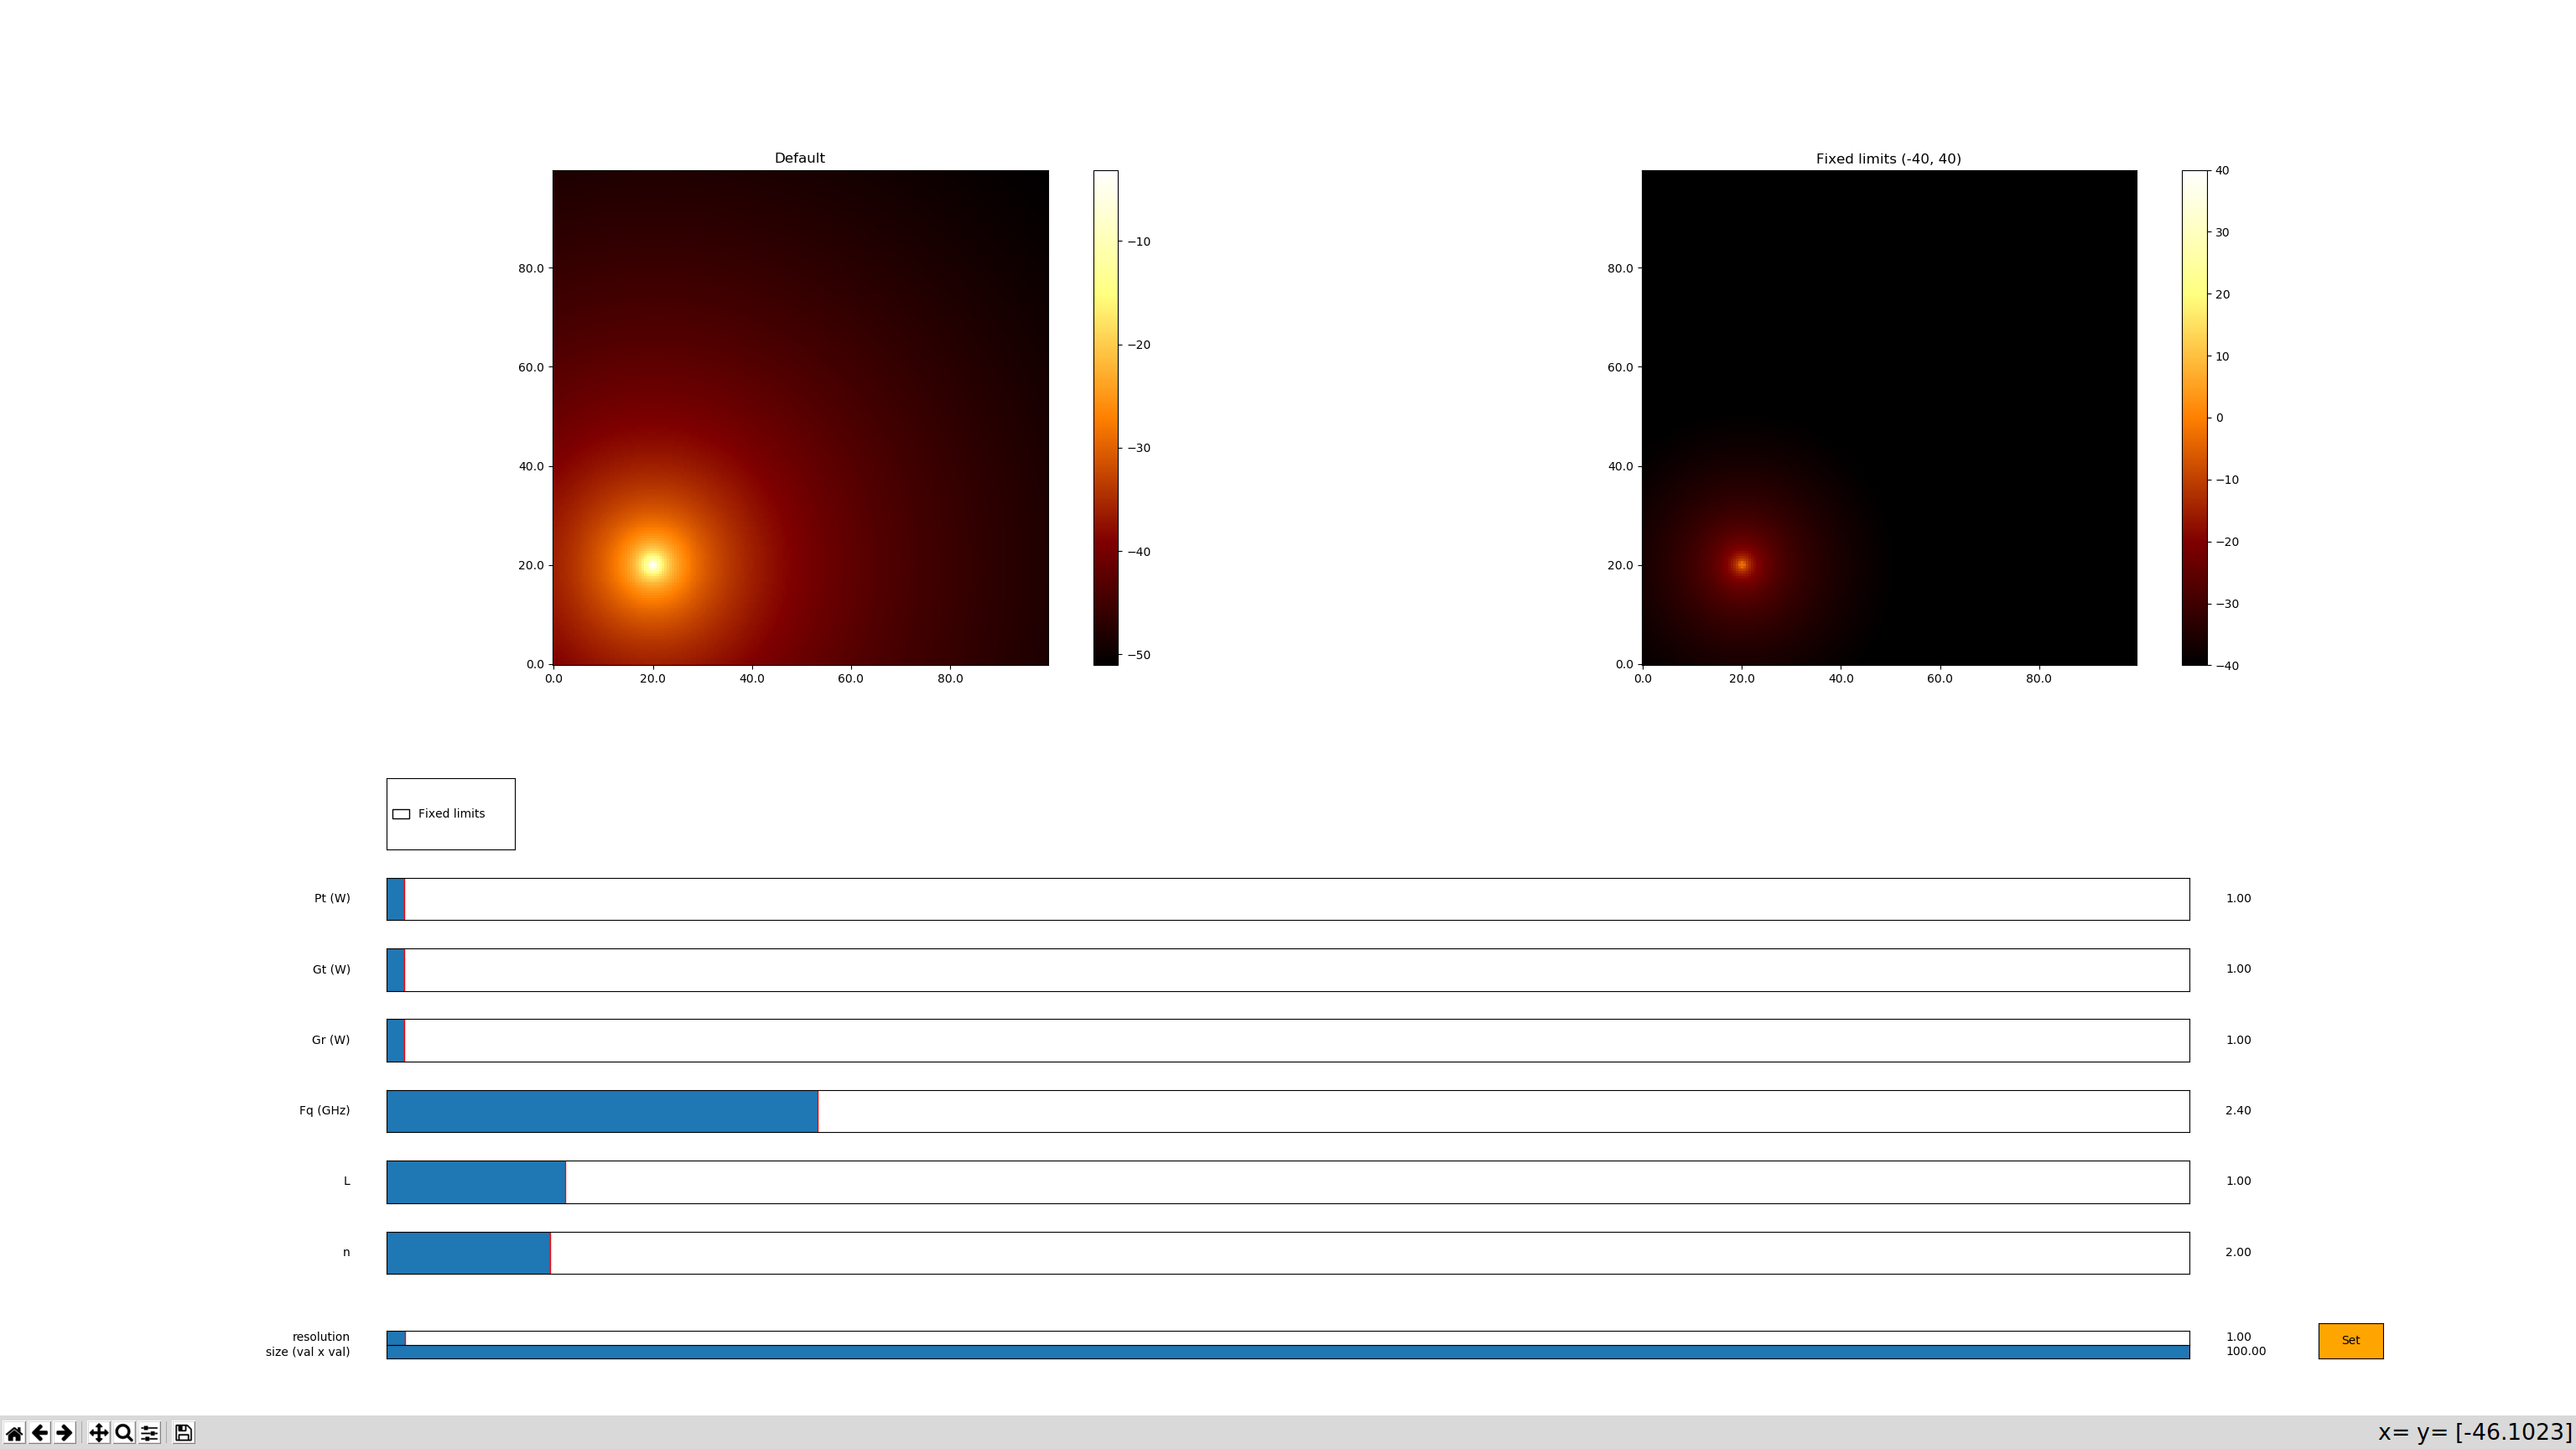
\includegraphics[height=8cm]{imagenes/cap4/7_Friss_endGUI.png}
    \end{center}
	\caption[Versión final de la interfaz]{Versión final de la interfaz}
	\label{fig:friis_end_app}
\end{figure}

Cabe destacar que, por motivos de desarrollo, no se agregó la parte de generación dinámica de obstáculos a la aplicación, ya que esta se desarrollo como un extra al final del \ac{TFG}.\\

\newpage
\section{Integración conjunta}
\label{sec:integration}

La integración conjunta engloba la parte final del proyecto, es la fase donde se juntaron las secciones anteriores, con el fin de generar el entorno deseado para resolver el problema.\\

El objetivo, a parte de llevar a cabo la tarea encomendada, comprobar y comparar los distintos algoritmos entre sí, a través de diversas métricas de rendimiento.\\

\subsection{Primeros pasos}
\label{subsec:primeros_pasos}

(intro)\\

(servidor de datos)\\

(heatmap en rviz)\\

\subsection{Algoritmos}
\label{subsec:algoritmos}

(intro)\\

(manual)\\

(manual optimizado)\\

(Q-Learning)\\

\subsection{Métricas empleadas}
\label{subsec:metricas}

(intro)\\

(mapa de posiciones)\\

(mapa de trayectorias)\\

(plots de entrenamiento)\\

(plots comparativos)\\

\subsection{Experimentos y resultados}
\label{subsec:experimentos_resultados}

(intro y señal estática)\\

(12x12)\\

(30x30)\\

(mismo mapa distinta señal)\\

\subsection{Experimentos con obstáculos}
\label{subsec:experimentos_obstaculos}

(intro)\\

(resultados)\\

